%-----------------------------------------------------------
\section{Architecture des visuels Power BI}
\label{sec:archi-powerbi}
%-----------------------------------------------------------

Power~BI est conçu autour d’une architecture de visualisation ouverte et extensible.  
Chaque visuel — graphique, jauge, carte ou autre — est rendu côté client à partir d’un DataView spécifique, généré automatiquement à partir du modèle de données filtré, via du code JavaScript/TypeScript exécuté dans Power~BI Desktop ou dans le service web \parencite{MicrosoftOpenVis2015}.  
Depuis 2015, Microsoft propose non seulement une panoplie de visuels « core » (natifs), mais permet aussi l’importation de visuels additionnels développés par la communauté ou des éditeurs tiers \parencite{MicrosoftMarketplace2016}.  
Cette ouverture repose sur des standards web — « en s’appuyant sur des standards ouverts d’Internet et des bibliothèques open-source comme D3.js », note Microsoft \parencite{MicrosoftD3Blog2017} — et se matérialise sur GitHub où le code source de nombreux visuels natifs est publié \parencite{GitHubPowerBISamples2024}.  
L’API publique a évolué de la branche 5.10 à la version stable 6.1.2 (26 mai 2025), qui introduit un DOM sécurisé ainsi que la Rendering Events API, renforçant la cohérence entre ouverture et sécurité \parencite{MicrosoftApiChangelog2025}.

Cette section examine d’abord le fonctionnement interne d’un visuel Power BI — de son chargement sécurisé à son intégration interactive — avant de présenter la plateforme AppSource, qui permet d’étendre les visuels disponibles sans développement.

\begin{figure}[h]
  \centering
  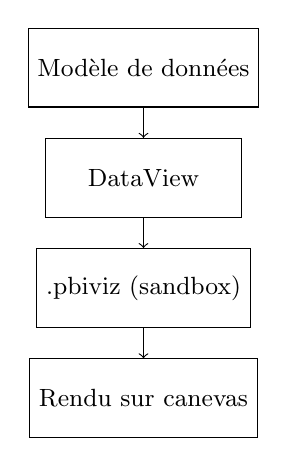
\begin{tikzpicture}[node distance=1.4cm, every node/.style={font=\small}]
    % Nodes
    \node (model) [draw, rectangle, minimum width=2.5cm, minimum height=1cm] {Modèle de données};
    \node (dataview) [below of=model, draw, rectangle, minimum width=2.5cm, minimum height=1cm] {DataView};
    \node (pbiviz) [below of=dataview, draw, rectangle, minimum width=2.5cm, minimum height=1cm] {.pbiviz (sandbox)};
    \node (canvas) [below of=pbiviz, draw, rectangle, minimum width=2.5cm, minimum height=1cm] {Rendu sur canevas};
    % Arrows
    \draw[->] (model) -- (dataview);
    \draw[->] (dataview) -- (pbiviz);
    \draw[->] (pbiviz) -- (canvas);
  \end{tikzpicture}
  \caption{Architecture simplifiée d’un visuel Power~BI personnalisé}
  \label{fig:archi-visuel}
\end{figure}

%-----------------------------------------------------------
\subsection{Visual container et bac à sable}
\label{subsec:sandbox}
%-----------------------------------------------------------

Qu’il soit natif ou personnalisé, un visuel s’insère dans le canevas du rapport et interagit avec le modèle de données via des rôles prédéfinis.  
Chaque visuel reçoit, du moteur Power BI, les données filtrées qui lui sont attribuées (colonnes, mesures, hiérarchies), puis exécute son propre code de rendu.  
Pour les visuels custom, ce code est empaqueté dans un fichier .pbiviz contenant scripts, styles et manifeste \parencite{MicrosoftPbivizDocs2023}.  
Power BI exécute alors le visuel dans un bac à sable sécurisé (sandbox) : une iframe isolée du reste du rapport \parencite{OkVizSandbox2022}.  
Le visuel n’accède ni aux autres visuels ni au modèle global ; il ne « voit » que les champs explicitement liés par l’utilisateur.  
Depuis la mise à jour 2.140 (février 2024), tout visuel — privé (organizational visual) ou destiné à AppSource — est audité par l’option pbiviz package --certification-audit de powerbi-visuals-tools ≥ 6.1 : les appels réseau (fetch, XMLHttpRequest, WebSockets) et l’évaluation dynamique de code (eval, Function) sont bloqués, et l’exécution est interrompue au-delà d’environ 120 s de CPU ou de 230 Mio de mémoire \parencite{MicrosoftCertificationGuide2025}.  
Ces garde-fous empêchent qu’un code malveillant puisse lire ou exfiltrer des données sans autorisation \parencite{MediumSecurityPBI2023}.

%-----------------------------------------------------------
\subsection{Interactions et intégration}
\label{subsec:interactions}
%-----------------------------------------------------------

Malgré cet isolement technique, les visuels s’intègrent pleinement dans l’expérience interactive globale.  
Un visuel personnalisé correctement développé se comporte exactement comme un visuel natif : il réagit aux filtres, autorise le cross-highlight (mise en surbrillance croisée) et expose des options de mise en forme dans le panneau Format \parencite{MicrosoftCustomVisGuide2024}.  
Lorsqu’un utilisateur clique, par exemple, sur une barre d’histogramme, le moteur Power BI propage l’événement de sélection aux autres visuels.  
Si le développeur a implémenté l’API ISelectionManager, son visuel peut émettre et recevoir ces événements ; il peut également recourir à ITooltipService pour les infobulles contextuelles ou à ILocalizationManager pour l’internationalisation, de sorte que l’intégration fonctionnelle et linguistique demeure uniforme \parencite{MicrosoftSelectionAPI2024, MicrosoftTooltipAPI2024}.  

La différence fondamentale reste donc interne : les visuels natifs font partie du produit et peuvent exploiter des API internes non exposées, tandis que les visuels personnalisés s’appuient uniquement sur l’API publique du SDK, avec les restrictions de sécurité détaillées en section~\ref{sec:sdk}.

%-----------------------------------------------------------
\subsection{AppSource comme catalogue de visuels certifiés}
\label{subsec:appsource}
%-----------------------------------------------------------

En complément des visuels natifs, Power BI propose une galerie en ligne nommée AppSource, accessible directement depuis l’interface de conception de rapports.  
Cette plateforme répertorie plusieurs centaines de visuels certifiés, gratuits ou payants, classés par thématique (cartographie, indicateurs, diagrammes spécialisés, etc.).  
Les utilisateurs peuvent y intégrer des composants supplémentaires sans compétence de développement, ce qui en fait une solution courante lorsqu’un besoin spécifique n’est pas couvert par les visuels standards.  
Toutefois, ces visuels restent limités à ce que les éditeurs tiers ont déjà publié, et leur personnalisation est restreinte.  
Dans le cadre de ce travail, AppSource est considéré comme une ressource de référence — utile à des fins de comparaison fonctionnelle —, mais le projet se concentre sur la création de composants ad hoc conçus pour un besoin métier spécifique, sans visée de diffusion publique via le store.
